%!TEX root=Principal.tex
\chapter{RESULTADOS E DISCUSSÕES}
\label{cap:resultados}
Foram selecionados 39 pessoas foram selecionadas para realizar o teste de interação com o robô em um ambiente doméstico, conforme apresentado na figura~\ref{fig:cenario}. O perfil dos usuários selecionados atendem o escopo do projeto enviado do comitê de ética sobre o registro CAAE: 70057117.0.0000.5508. A tabela~\ref{tab:perfilamostra} apresenta as informações básicas sobre os usuários selecionados para realizar os testes.

\begin{table}[!ht]
	\caption{Perfis dos usuários que realizaram o teste.}
	\label{tab:perfilamostra}
	\centering
	\begin{tabular}{c | c | c | c | c | c | c | c}
        \hline
        Idade & Altura & Gênero & Feição & Sociável? & Óculos & Cabelo & Etnia \\
         &  &  &  &  & de Grau? & Comprido? &  \\
        \hline
        31 & 1.74 & Masculino & Normal & Sim & Não & Não & Branca \\
        \hline
        24 & 1.80 & Masculino & Sorridente & Sim & Sim & Não & Branca \\
        \hline
        26 & 1.70 & Masculino & Sorridente & Sim & Não & Não & Parda \\
        \hline
        19 & 1.70 & Masculino & Normal & Não & Não & Não & Branca \\
        \hline
        20 & 1.68 & Feminino & Sorridente & Sim & Sim & Sim & Branca \\
        \hline
        20 & 1.63 & Feminino & Normal & Sim & Sim & Não & Parda \\
        \hline
        20 & 1.68 & Masculino & Sorridente & Sim & Sim & Não & Branca \\
        \hline
        20 & 1.80 & Masculino & Sorridente & Sim & Sim & Não & Branca \\
        \hline
        34 & 1.85 & Masculino & Normal & Sim & Não & Não & Branca \\
        \hline
        22 & 1.61 & Feminino & Séria/Fechada & Sim & Sim & Sim & Preta \\
        \hline
        23 & 1.80 & Masculino & Séria/Fechada & Não & Sim & Não & Branca \\
        \hline
        20 & 1.65 & Masculino & Sorridente & Sim & Sim & Não & Branca \\
        \hline
        24 & 1.68 & Masculino & Séria/Fechada & Sim & Não & Não & Branca \\
        \hline
        20 & 1.75 & Masculino & Sorridente & Não & Sim & Não & Branca \\
        \hline
        21 & 1.80 & Masculino & Normal & Não & Não & Não & Branca \\
        \hline
        22 & 1.72 & Masculino & Sorridente & Sim & Sim & Não & Branca \\
        \hline
        26 & 1.75 & Masculino & Sorridente & Sim & Não & Não & Branca \\
        \hline
        30 & 1.59 & Feminino & Normal & Sim & Não & Sim & Parda \\
        \hline
        27 & 1.83 & Masculino & Normal & Sim & Não & Não & Parda \\
        \hline
        24 & 1.78 & Masculino & Normal & Sim & Não & Não & Preta \\
        \hline
        42 & 1.78 & Masculino & Sorridente & Sim & Não & Sim & Branca \\
        \hline
        33 & 1.85 & Masculino & Sorridente & Sim & Sim & Não & Branca \\
        \hline
        24 & 1.70 & Masculino & Normal & Sim & Não & Não & Branca \\
        \hline
        24 & 1.76 & Masculino & Normal & Sim & Não & Não & Branca \\
        \hline
        18 & 1.63 & Masculino & Sorridente & Sim & Sim & Sim & Branca \\
        \hline
        33 & 1.75 & Masculino & Sorridente & Sim & Não & Não & Branca \\
        \hline
        22 & 1.67 & Feminino & Sorridente & Sim & Não & Não & Branca \\
        \hline
        22 & 1.67 & Masculino & Séria/Fechada & Sim & Não & Não & Preta \\
        \hline
        21 & 1.51 & Feminino & Normal & Não & Sim & Sim & Amarela \\
        \hline
        19 & 1.73 & Masculino & Normal & Sim & Não & Não & Branca \\
        \hline
        34 & 1.66 & Feminino & Sorridente & Não & Sim & Sim & Amarela \\
        \hline
        39 & 1.77 & Masculino & Normal & Sim & Não & Não & Branca \\
        \hline
        22 & 1.63 & Feminino & Normal & Sim & Não & Sim & Branca \\
        \hline
        19 & 1.80 & Masculino & Sorridente & Não & Não & Não & Branca \\
        \hline
        20 & 1.75 & Masculino & Normal & Sim & Não & Não & Branca \\
        \hline
        36 & 1.68 & Feminino & Normal & Sim & Não & Não & Branca \\
        \hline
        20 & 1.87 & Masculino & Normal & Sim & Sim & Não & Branca \\
        \hline
        40 & 1.74 & Feminino & Normal & Sim & Sim & Não & Branca \\
        \hline
        23 & 1.82 & Masculino & Normal & Sim & Não & Não & Branca \\
        \hline
	\end{tabular}
	\smallcaption{Fonte: O autor.}
\end{table}

A tabela~\ref{tab:perfilamostra} apresenta a informação declarada sobre todos os paritipantes do teste de para criação do classificador. Pode-se identificar os limites das variáveis dos parcipantes como, a idade mínima apresentada é de 18 anos e a máxima de 42 anos. A relação entre altura das pessoas, a menor estatura foi de 1,51 m contra 1,87 m da maior. Foram 29 homens e 10 mulheres na amostra, distribuídos entre funcionários e alunos da instituição de ensino. Todas essas informações obtidas através do questionário pré experimento são confrontadas com as informações do pós para análise.

Durante os testes com os 39 participantes, o foco foi entender como eles se sentiam em um cenário de interação doméstico enquanto o robô se aproximava deles. O sentimento foi traduzido em conforto e medo, através do questionário pós experimento. Confrontando algumas informações, foram gerados alguns gráficos como tentativa de entender o perfil do usuário e como classificá-lo posteriormente.

A figura~\ref{fig:confortogenero} apresenta a relação das informações sobre gênero dos participantes e o quanto ele se sentiu confortável na interação com o robô sendo o menor valor para totalmente desconfortável e o maior totalmente confortável.

\begin{figure}[ht!]
	\centering
	\begin{minipage}{0.65\textwidth}
		\caption{Conforto por gênero.}
		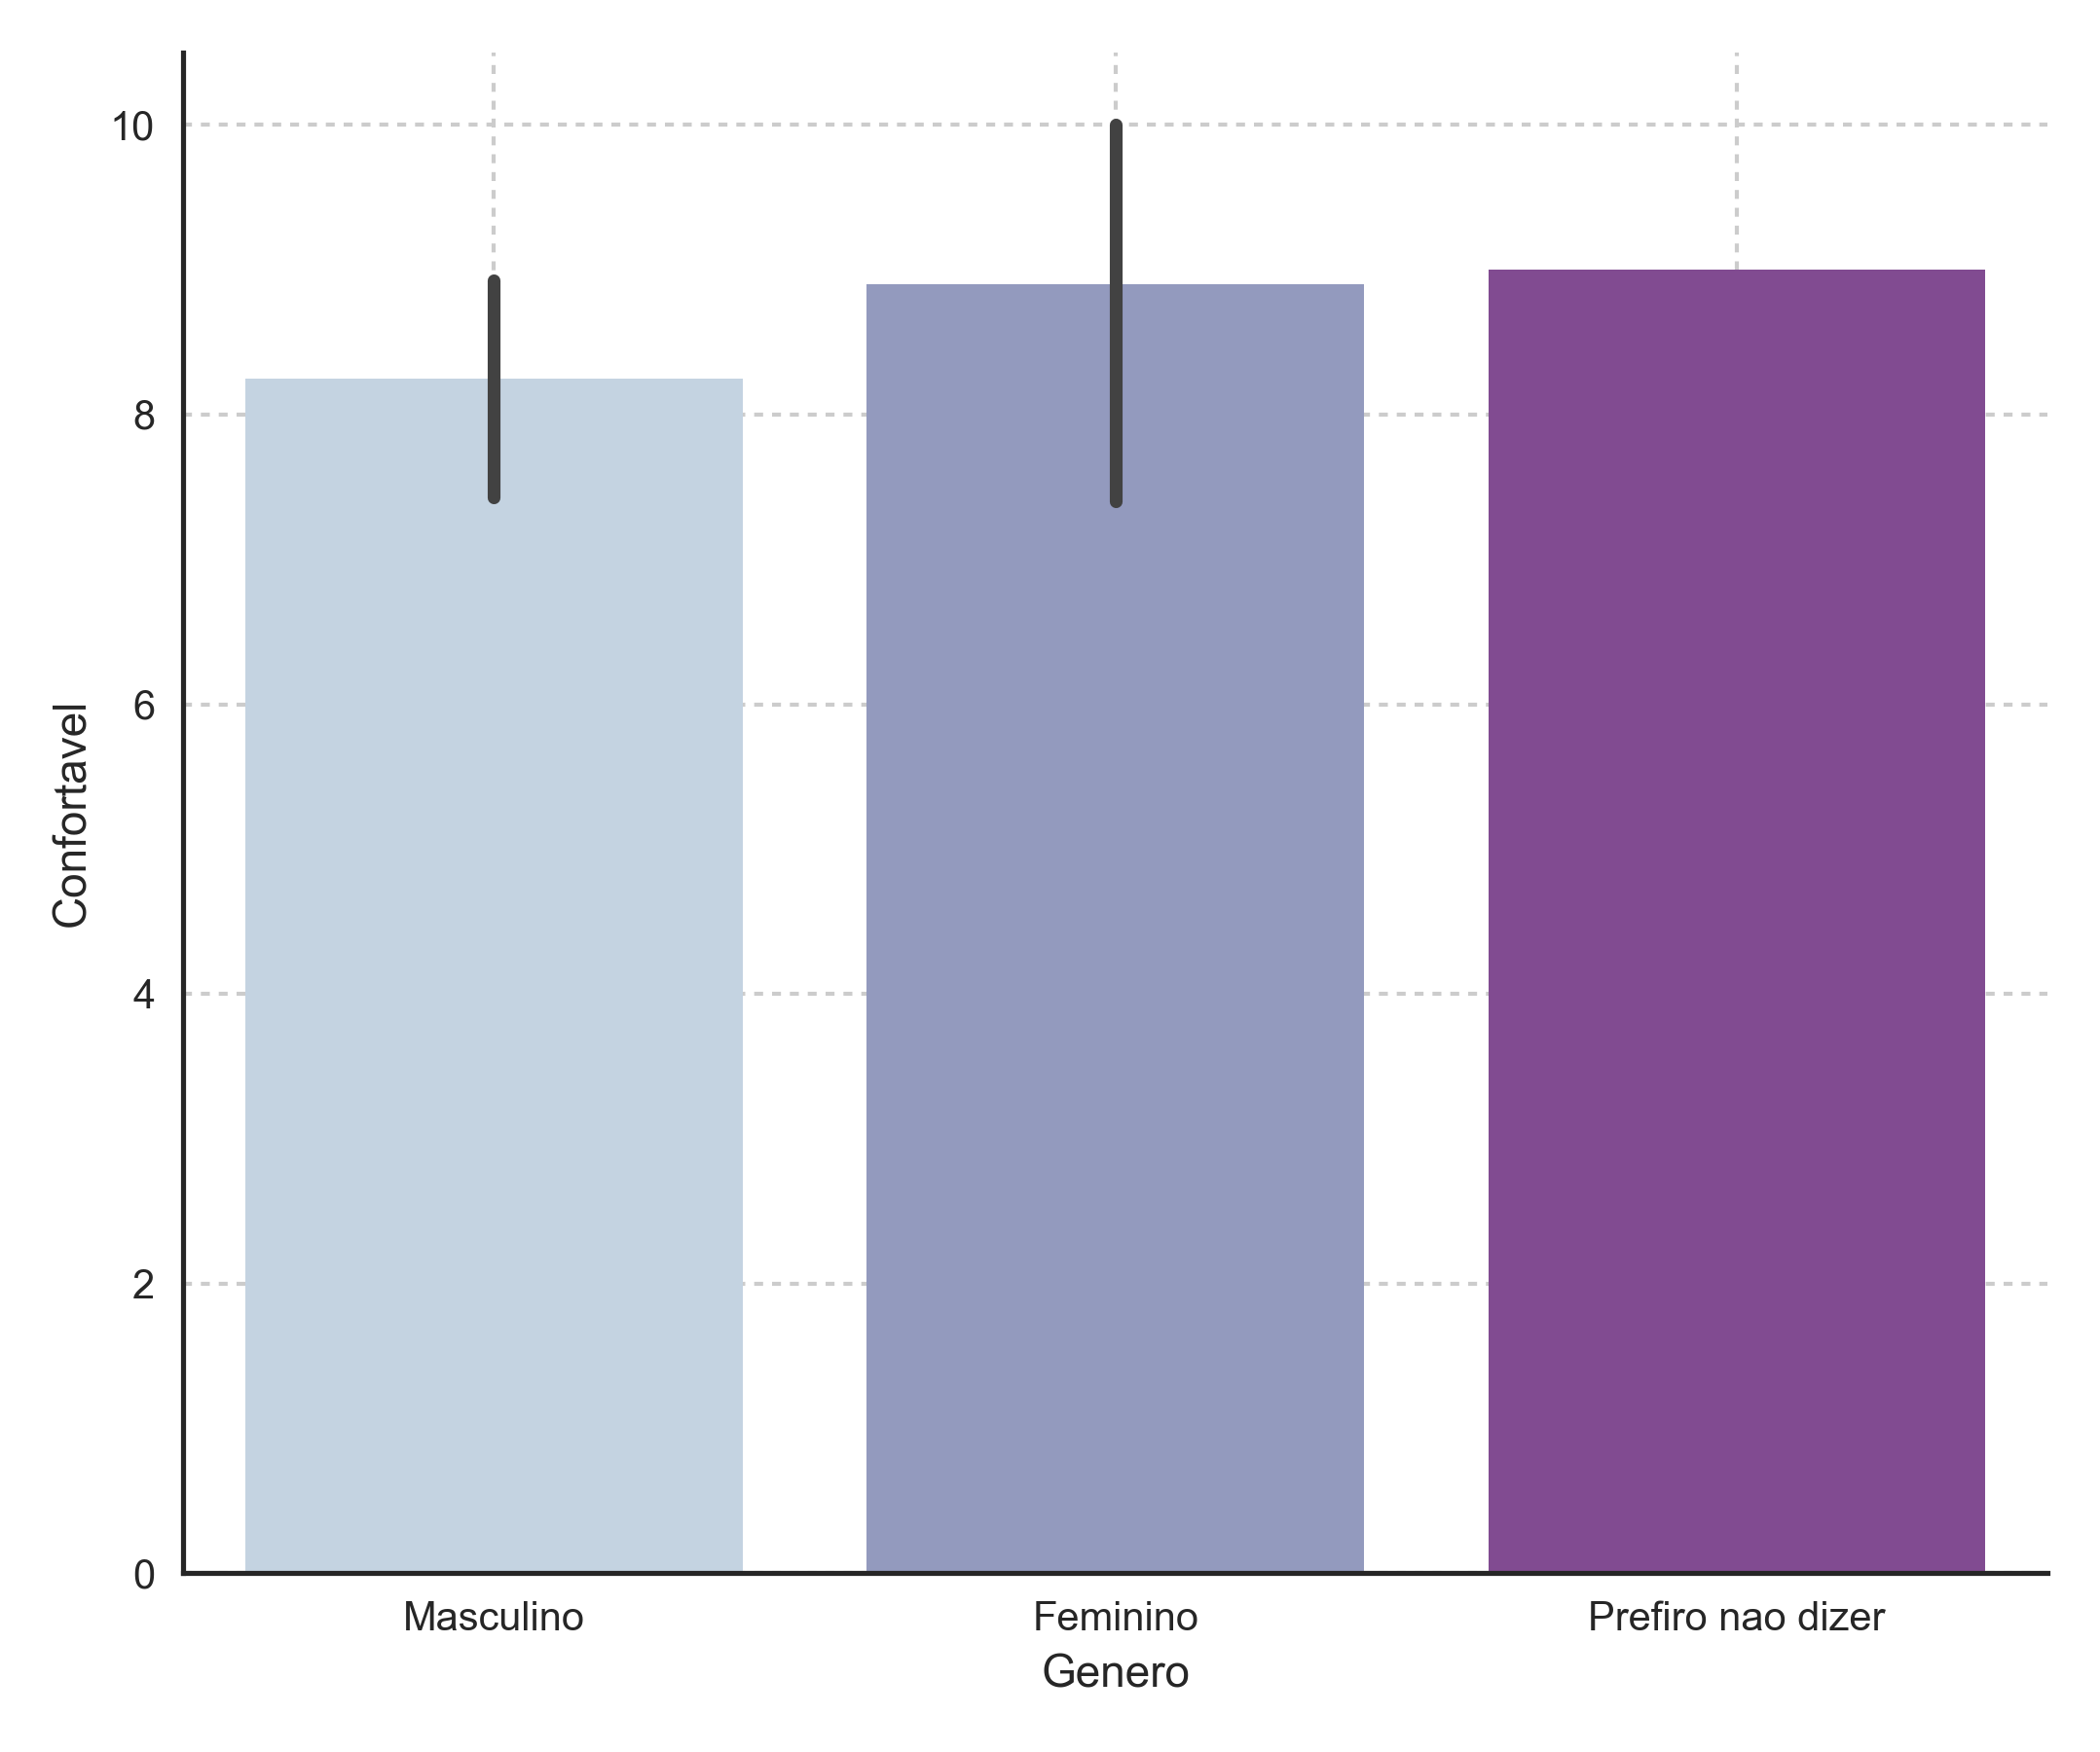
\includegraphics[width=\textwidth]{conforto_genero.png}
		\smallcaption{Fonte: O autor.}
		\label{fig:confortogenero}
	\end{minipage}
\end{figure}

Pode-se observar na figura~\ref{fig:confortogenero} que o gênero que se manteve mais confortável com o robô na aproximação foi o feminino. Isso ocorreu em grande parte devido a exibição das expressões faciais do robô. As participantes do gênero feminino acolheu o robô como uma criança ou pessoa meiga se aproximando dela. Outra variável que é comparada é a idade dos partipantes com o nível de conforto, apresentado na figura~\ref{fig:confortoidade}.

\begin{figure}[ht!]
	\centering
	\begin{minipage}{0.65\textwidth}
		\caption{Conforto por idade.}
		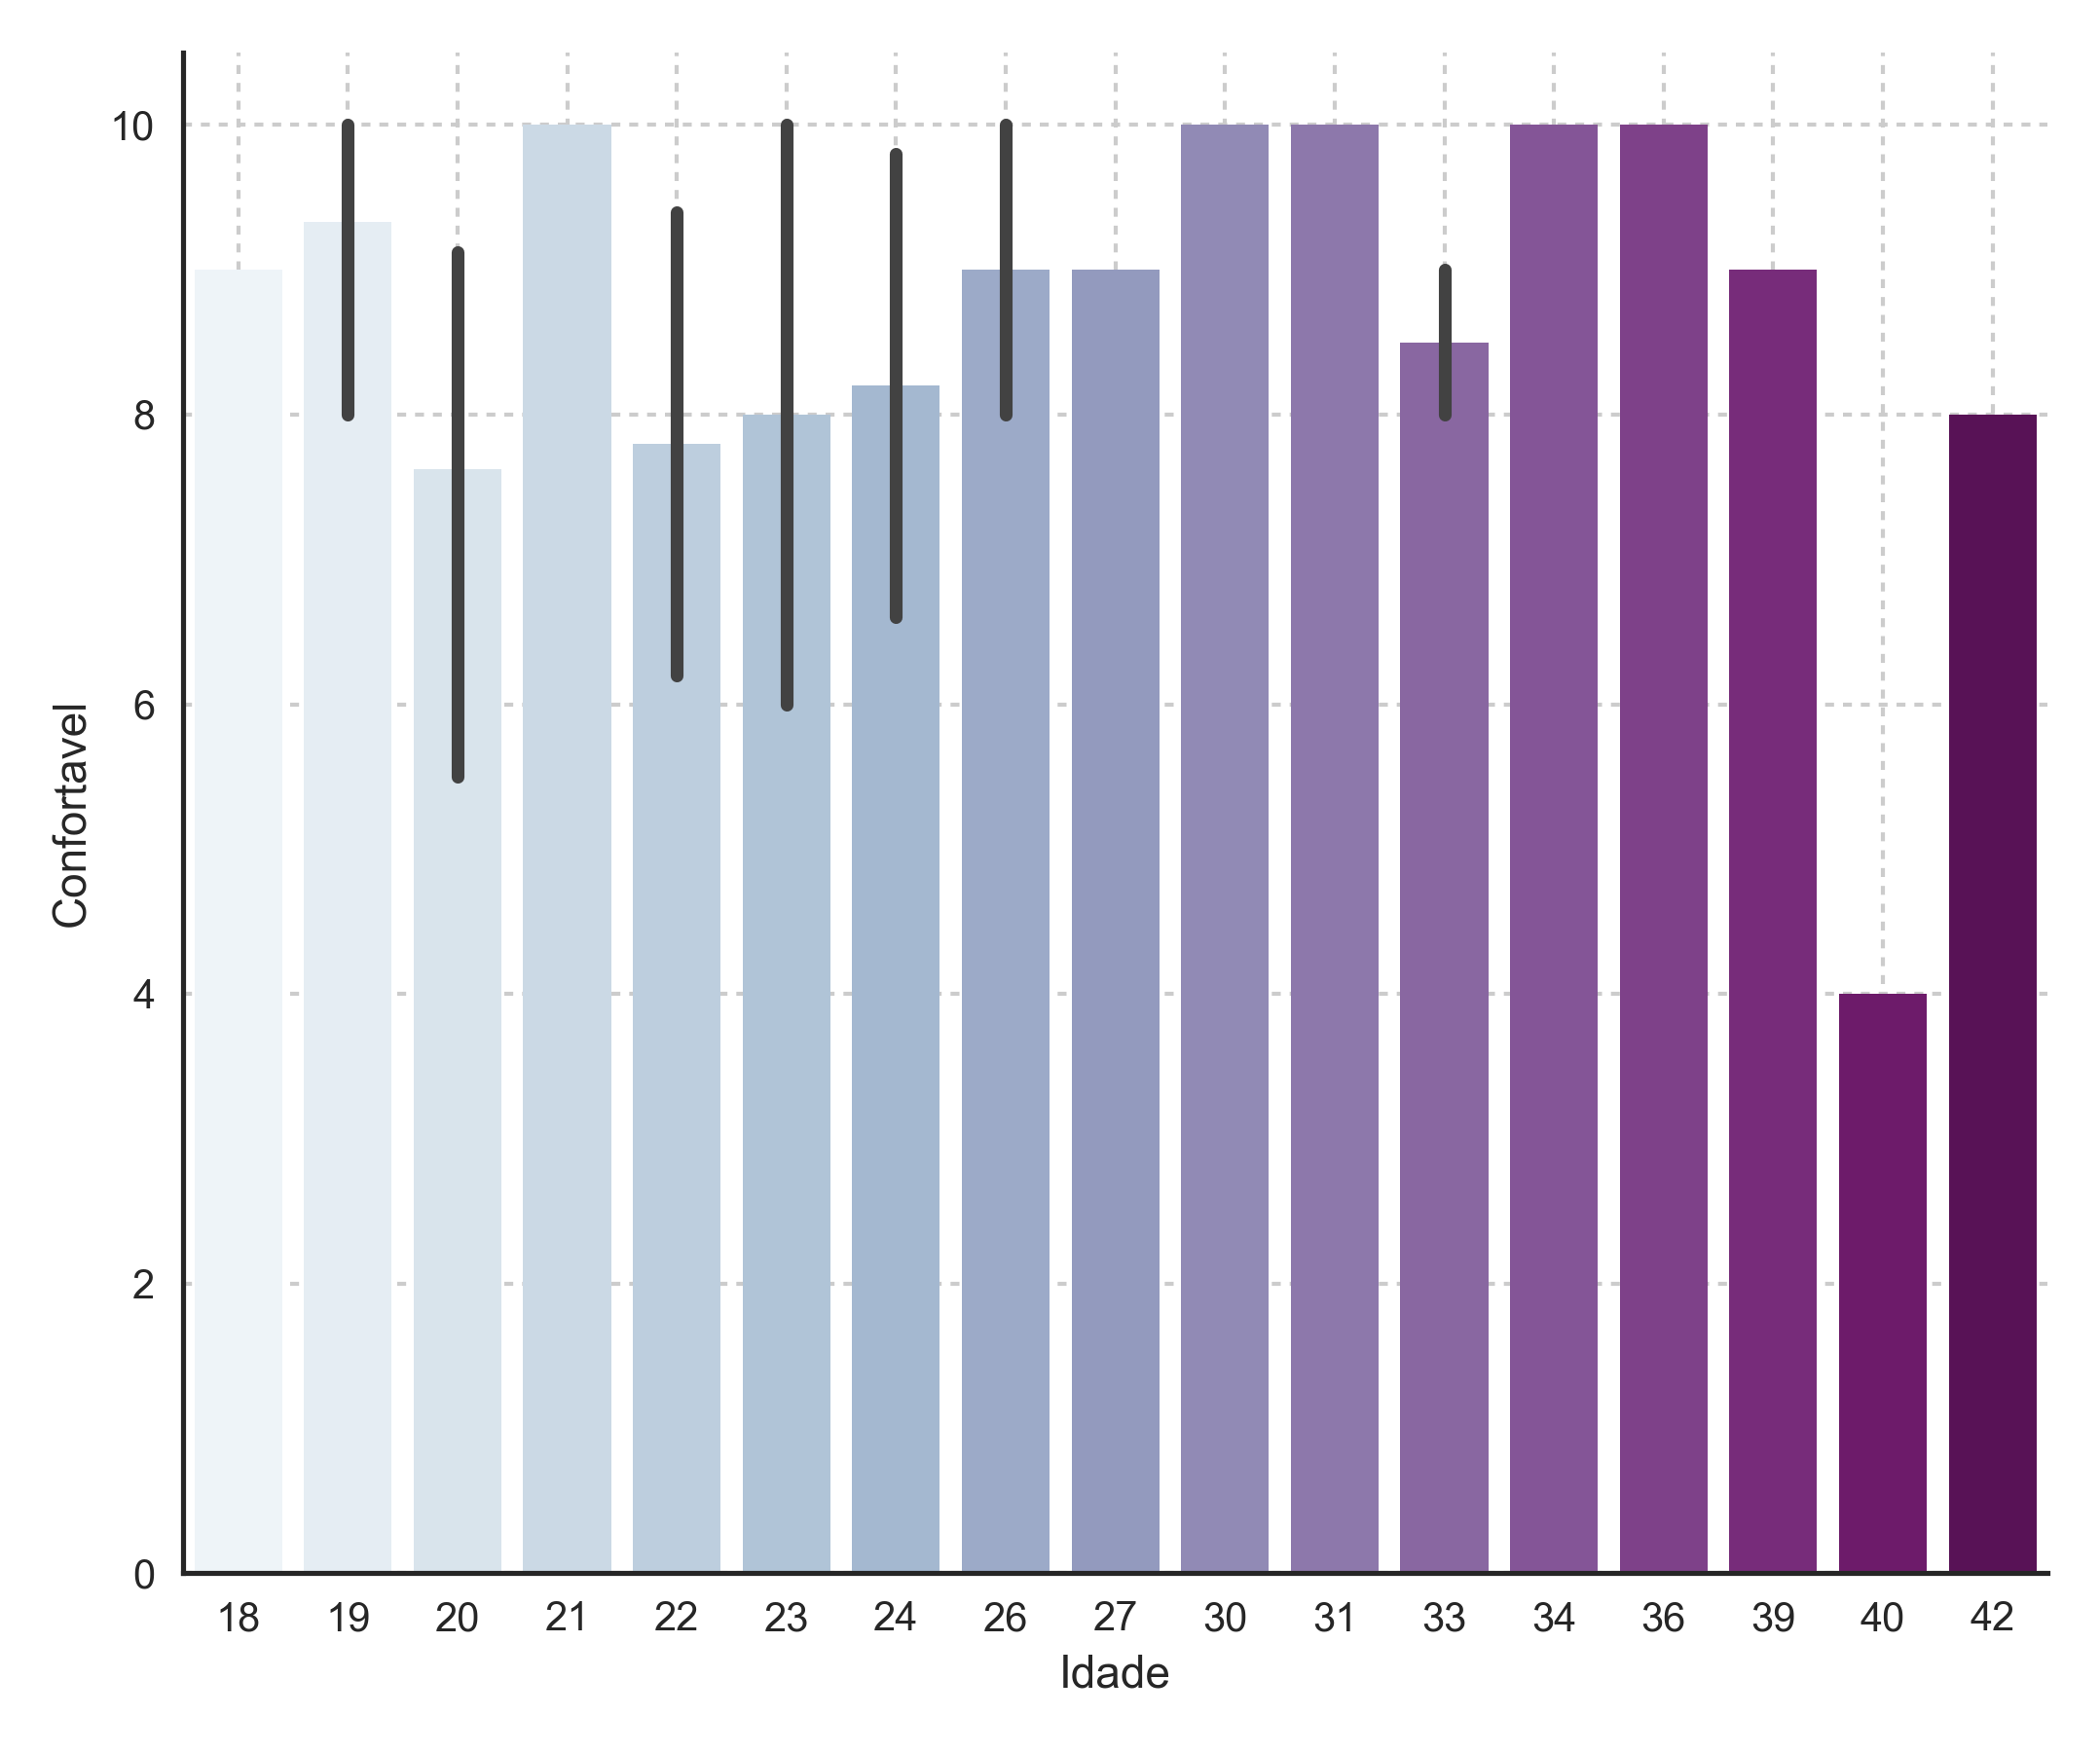
\includegraphics[width=\textwidth]{conforto_idade.png}
		\smallcaption{Fonte: O autor.}
		\label{fig:confortoidade}
	\end{minipage}
\end{figure}

Uma observação interessante é que apenas dois participantes apresentaram um nível de desconforto alto na aproximação do robô. Um participante de 20 e outro de 40 anos ficaram mais desconfortáveis com o robô, como observado na figura~\ref{fig:confortoidade}.

Na figura~\ref{fig:confortoposicao} é apresentada a relação entre o conforto do participante e a posição dele durante a interação, sentado ou em pé.

\begin{figure}[ht!]
	\centering
	\begin{minipage}{0.65\textwidth}
		\caption{Conforto por posição de interação.}
		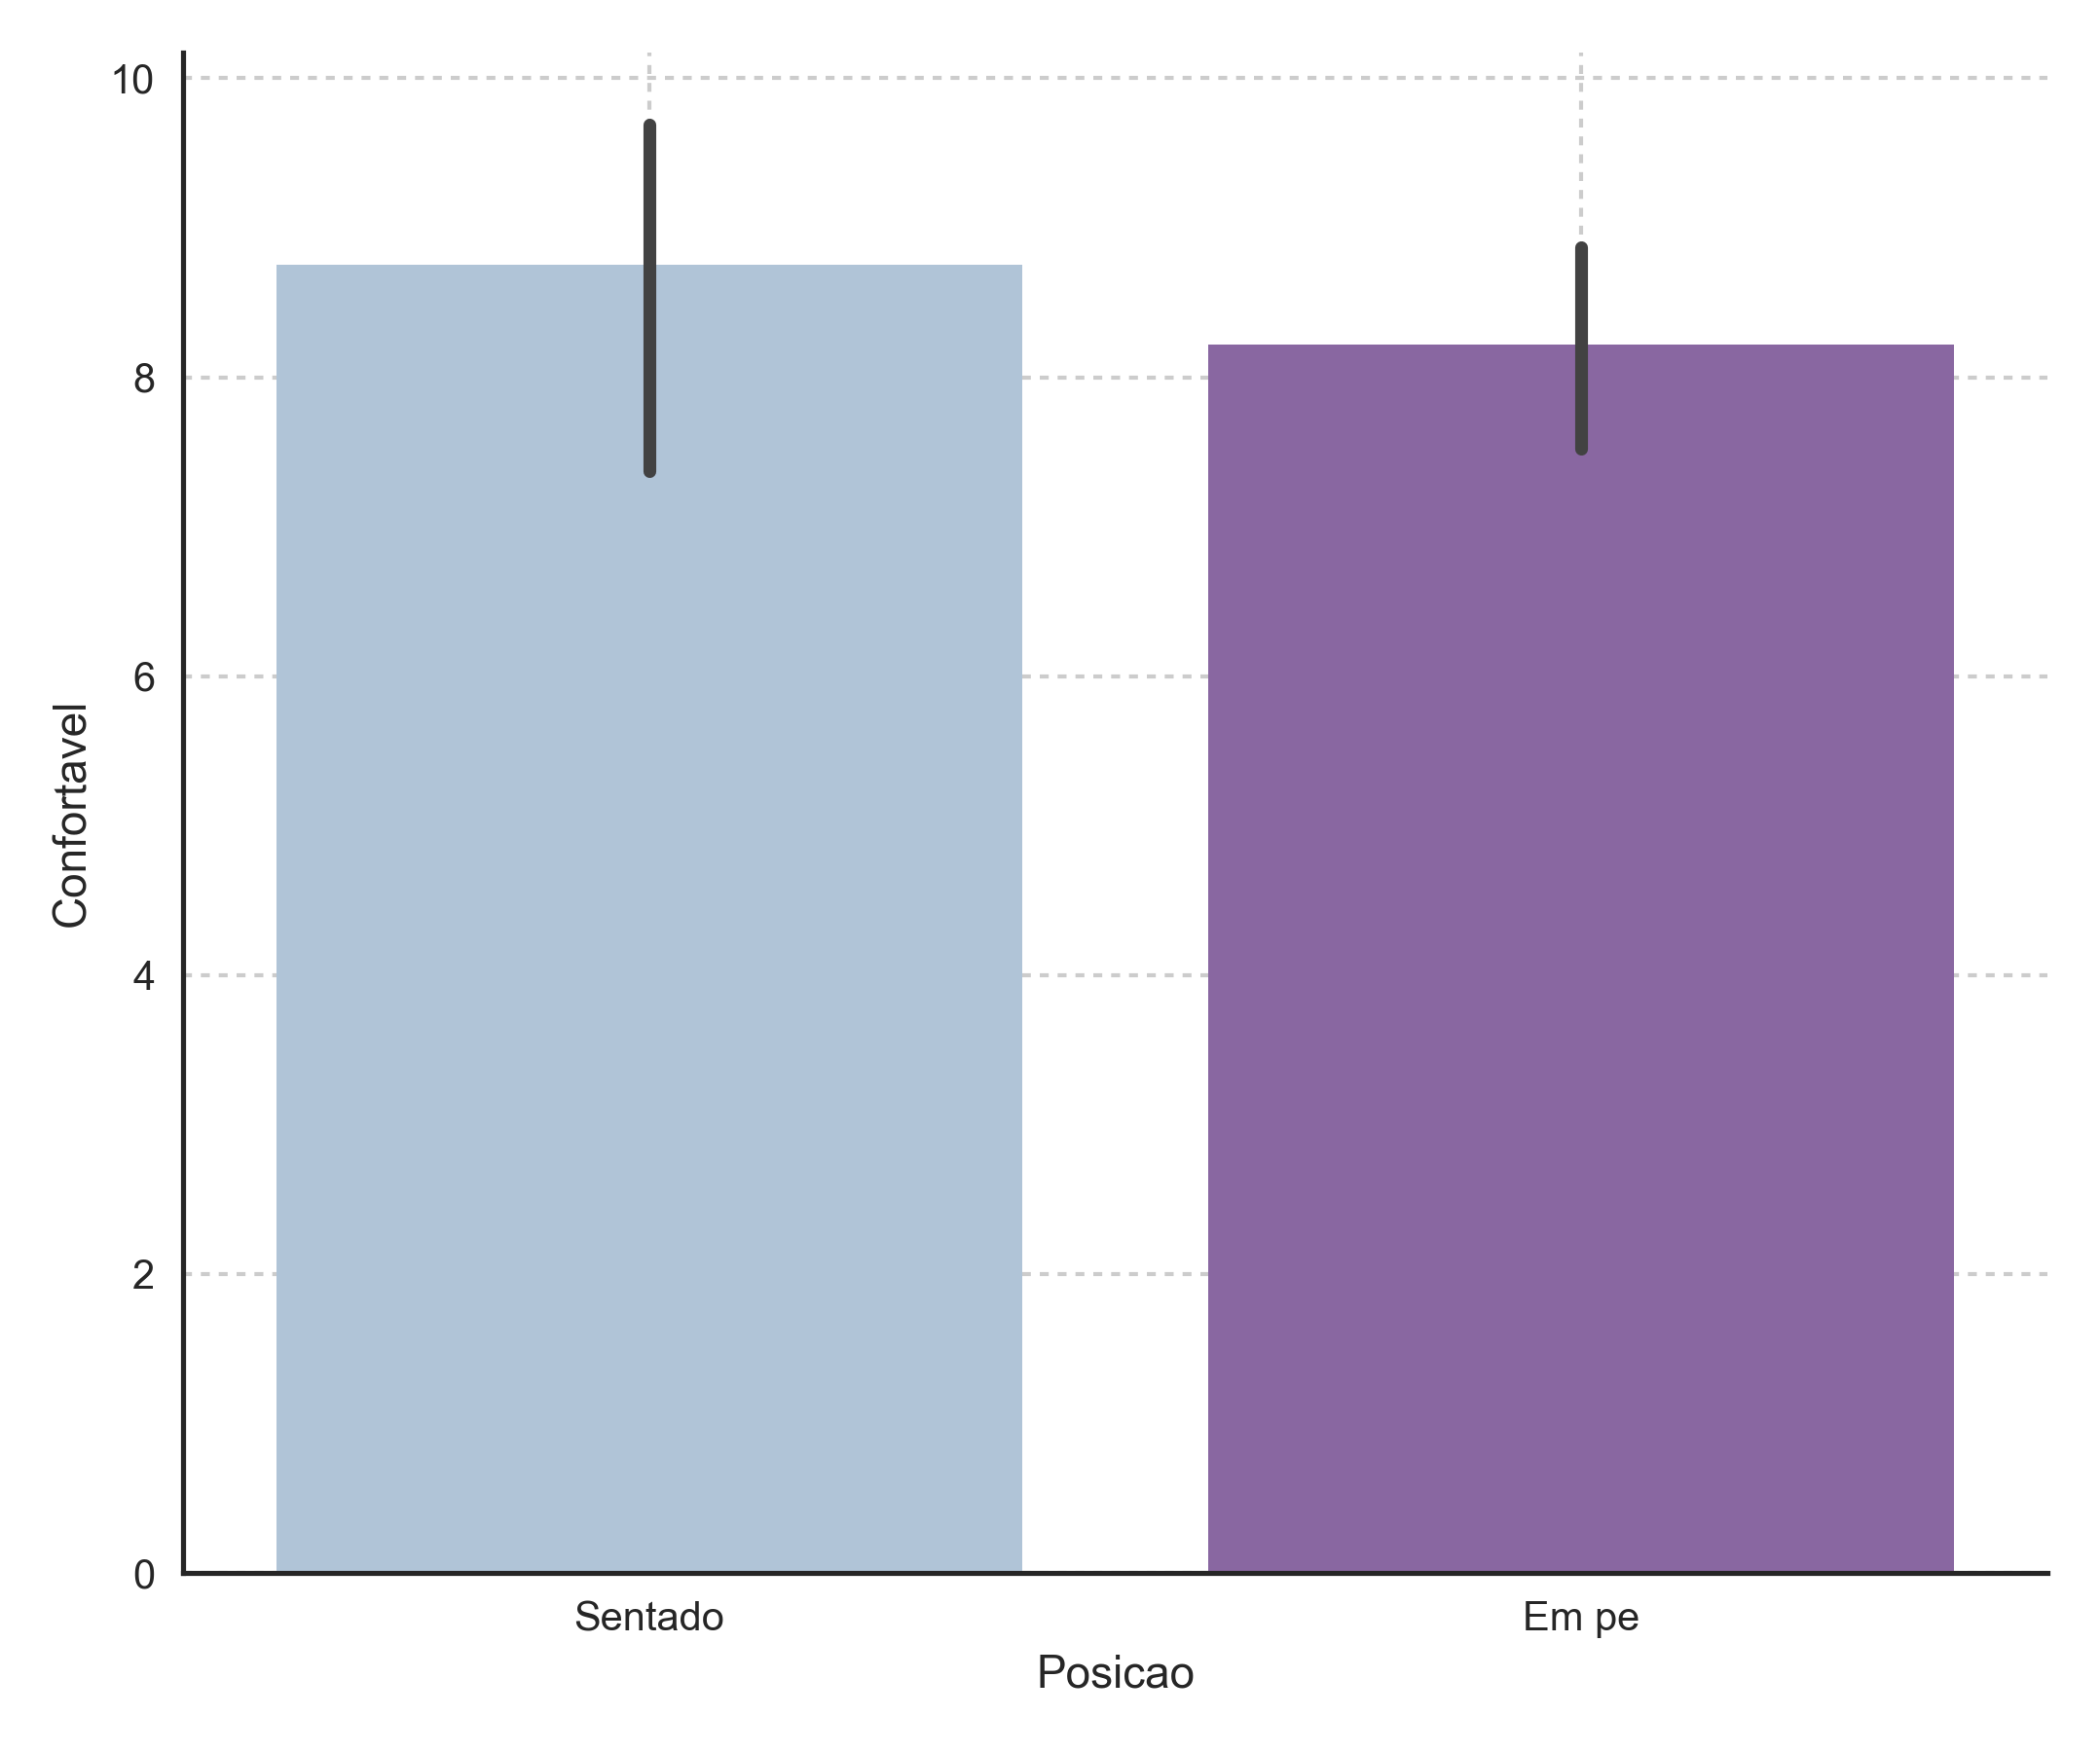
\includegraphics[width=\textwidth]{conforto_posicao.png}
		\smallcaption{Fonte: O autor.}
		\label{fig:confortoposicao}
	\end{minipage}
\end{figure}

É observado na figura~\ref{fig:confortoposicao} algo que foi observado diferente na competição da RoboCup, onde as pessoas sentadas sentiram maior desconforto. Nos testes, as pessoas que estavam sentadas durante a interação com o robô sentiram-se mais confortavéis do que as pessoas que estavam em pé. Esse é um fenômeno que pode ocorrer, pois o robô tocou no braço e barriga de alguns participantes que estavam em pé quando esticou o manipulador para chamar a atenção deles. Por último, é apresentado na figura~\ref{fig:confortosociavel} o nível de conforto dos participantes, dado a sua declaração de sociável ou não.

\begin{figure}[ht!]
	\centering
	\begin{minipage}{0.65\textwidth}
		\caption{Conforto por declaração de sociável.}
		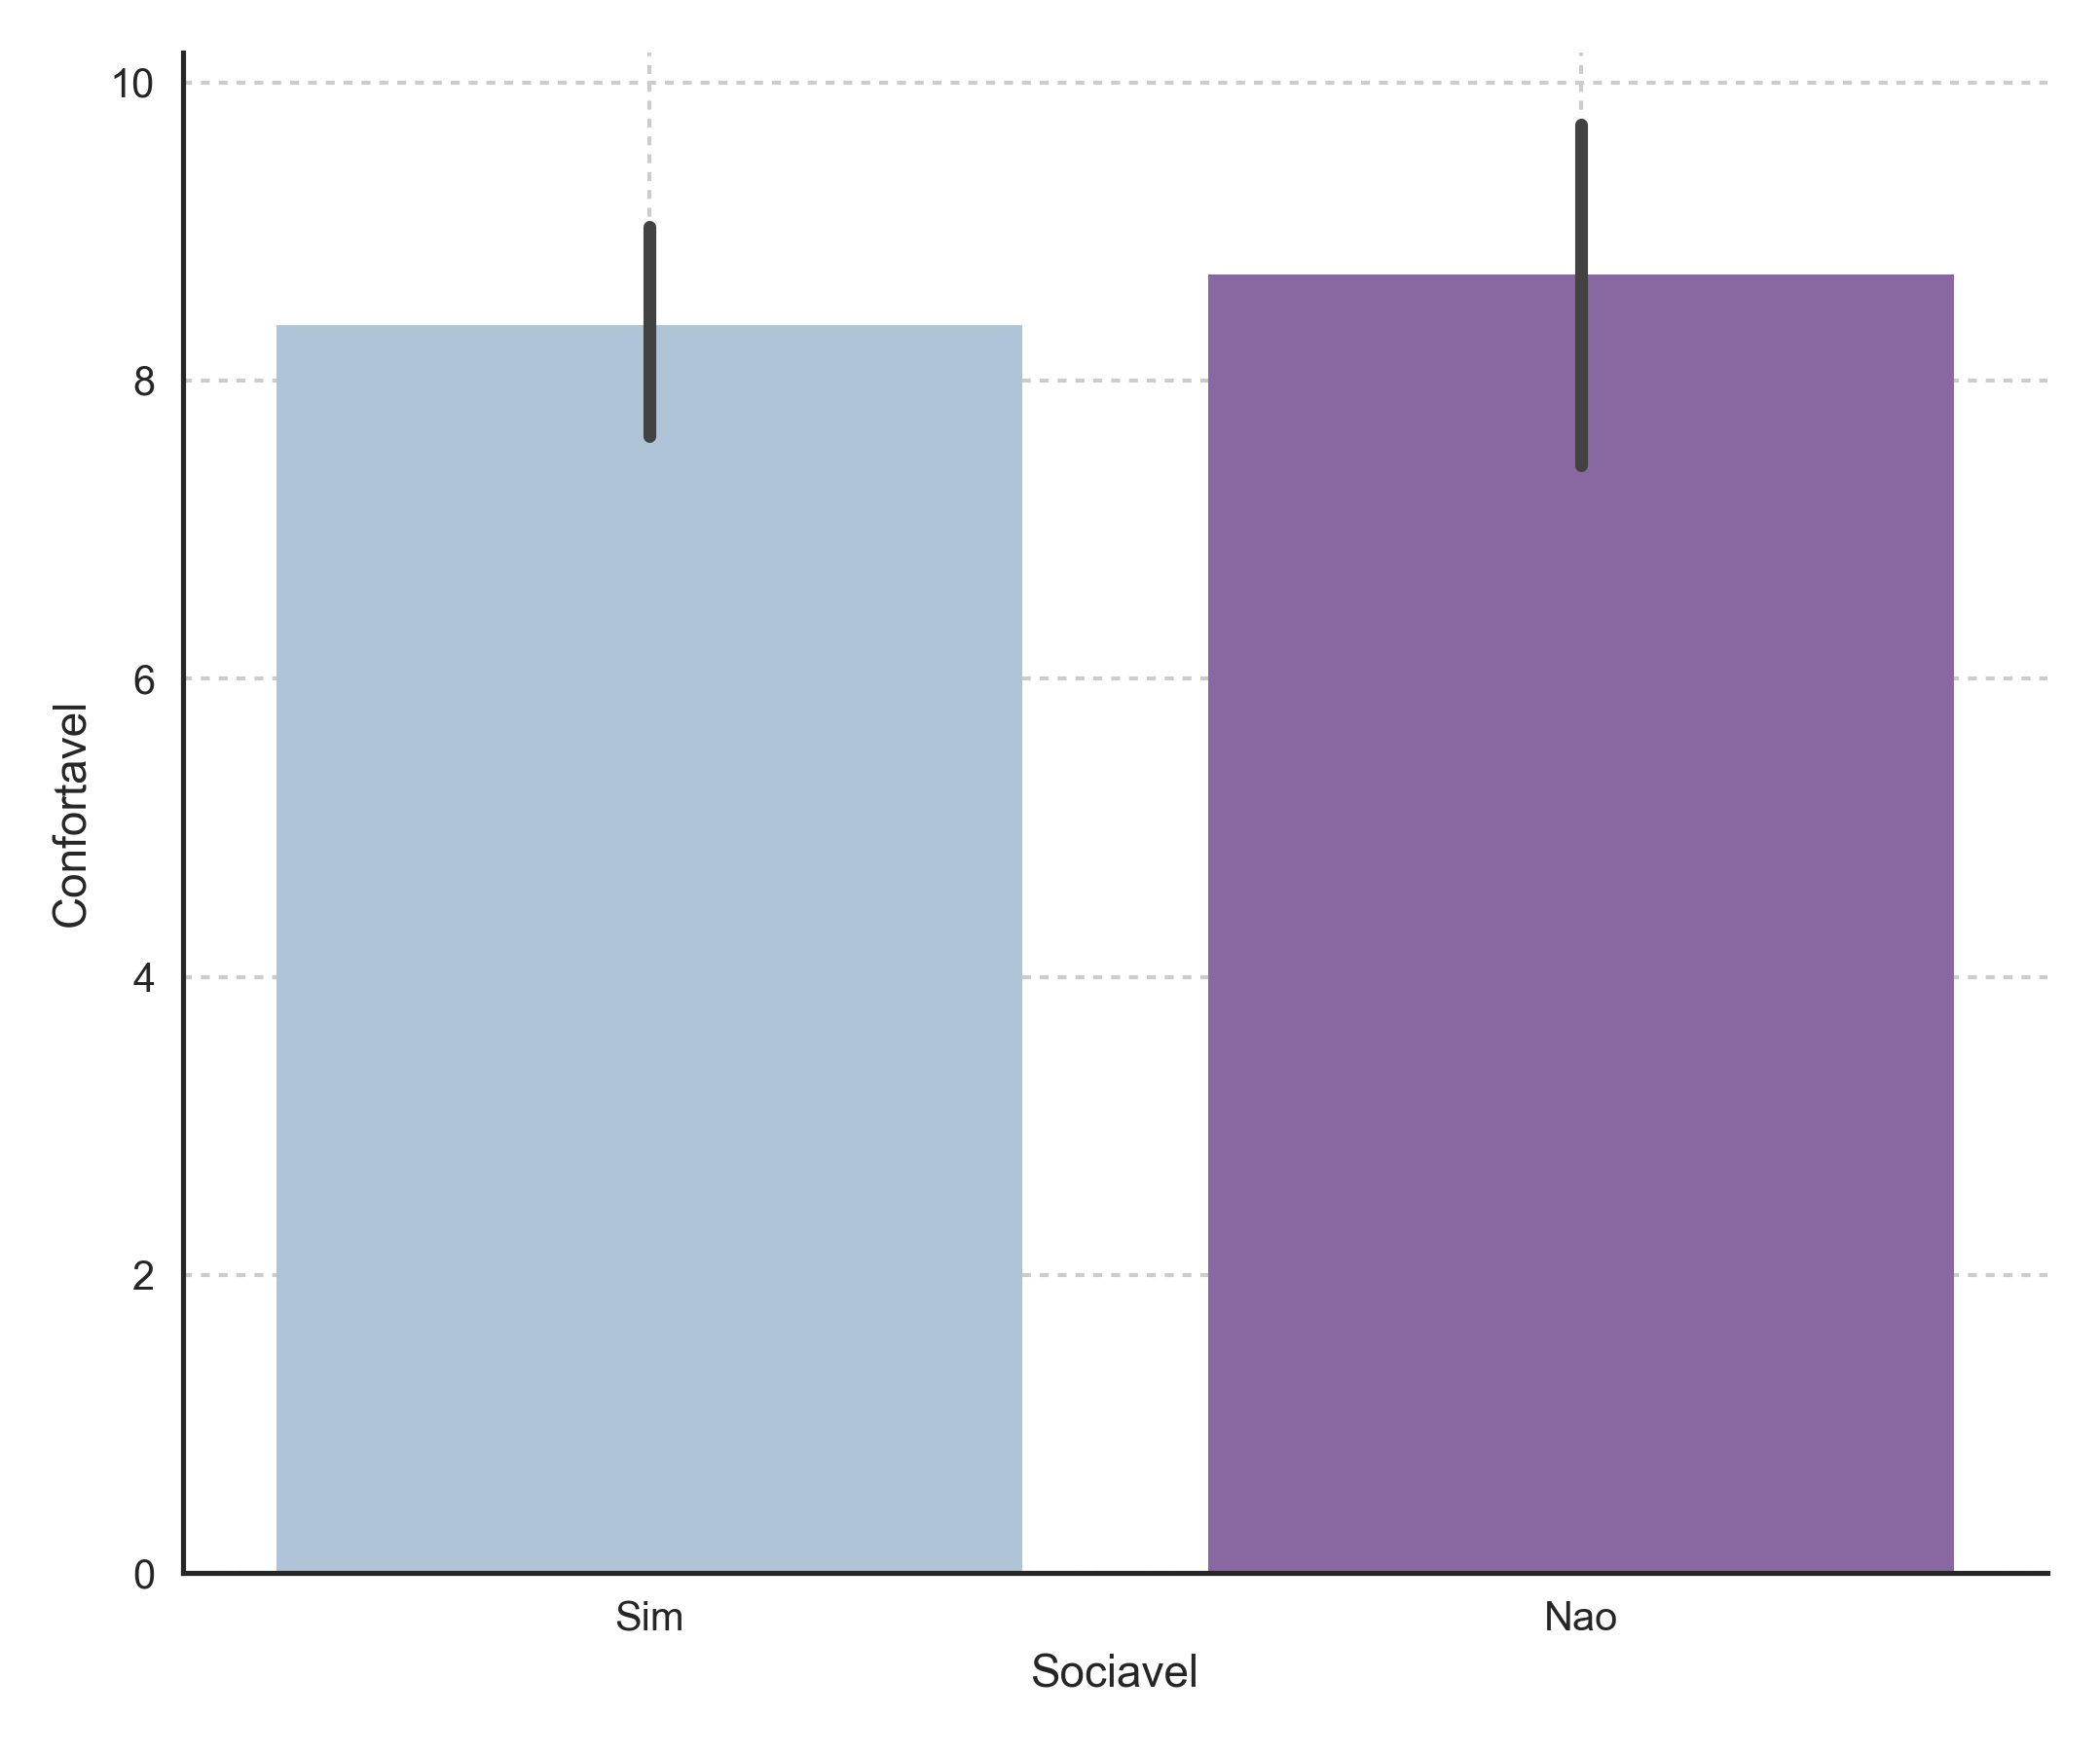
\includegraphics[width=\textwidth]{conforto_sociavel.png}
		\smallcaption{Fonte: O autor.}
		\label{fig:confortosociavel}
	\end{minipage}
\end{figure}

Mais um ponto interessante nessa análise feita através da figura~\ref{fig:confortosocial}. As pessoas declaradas como não sociáveis, foram as pessoas que mais se sentiram confortáveis durante toda a aproximação do robô. É um ponto interessante, pois se observar pela lógica, as pessoas sociáveis deveriam estar mais confortável e abertas a novas experiências.

A mesma análise para o conforto do usuário, foi realizada para a declaração de medo. Na escala da pergunta de medo o menor valor corresponde a totalmente com medo e o maior corresponde a totalmente sem medo. A figura~\ref{fig:medogenero} apresenta a relação entre o medo e o gênero do participante.

\begin{figure}[ht!]
	\centering
	\begin{minipage}{0.65\textwidth}
		\caption{Medo por gênero.}
		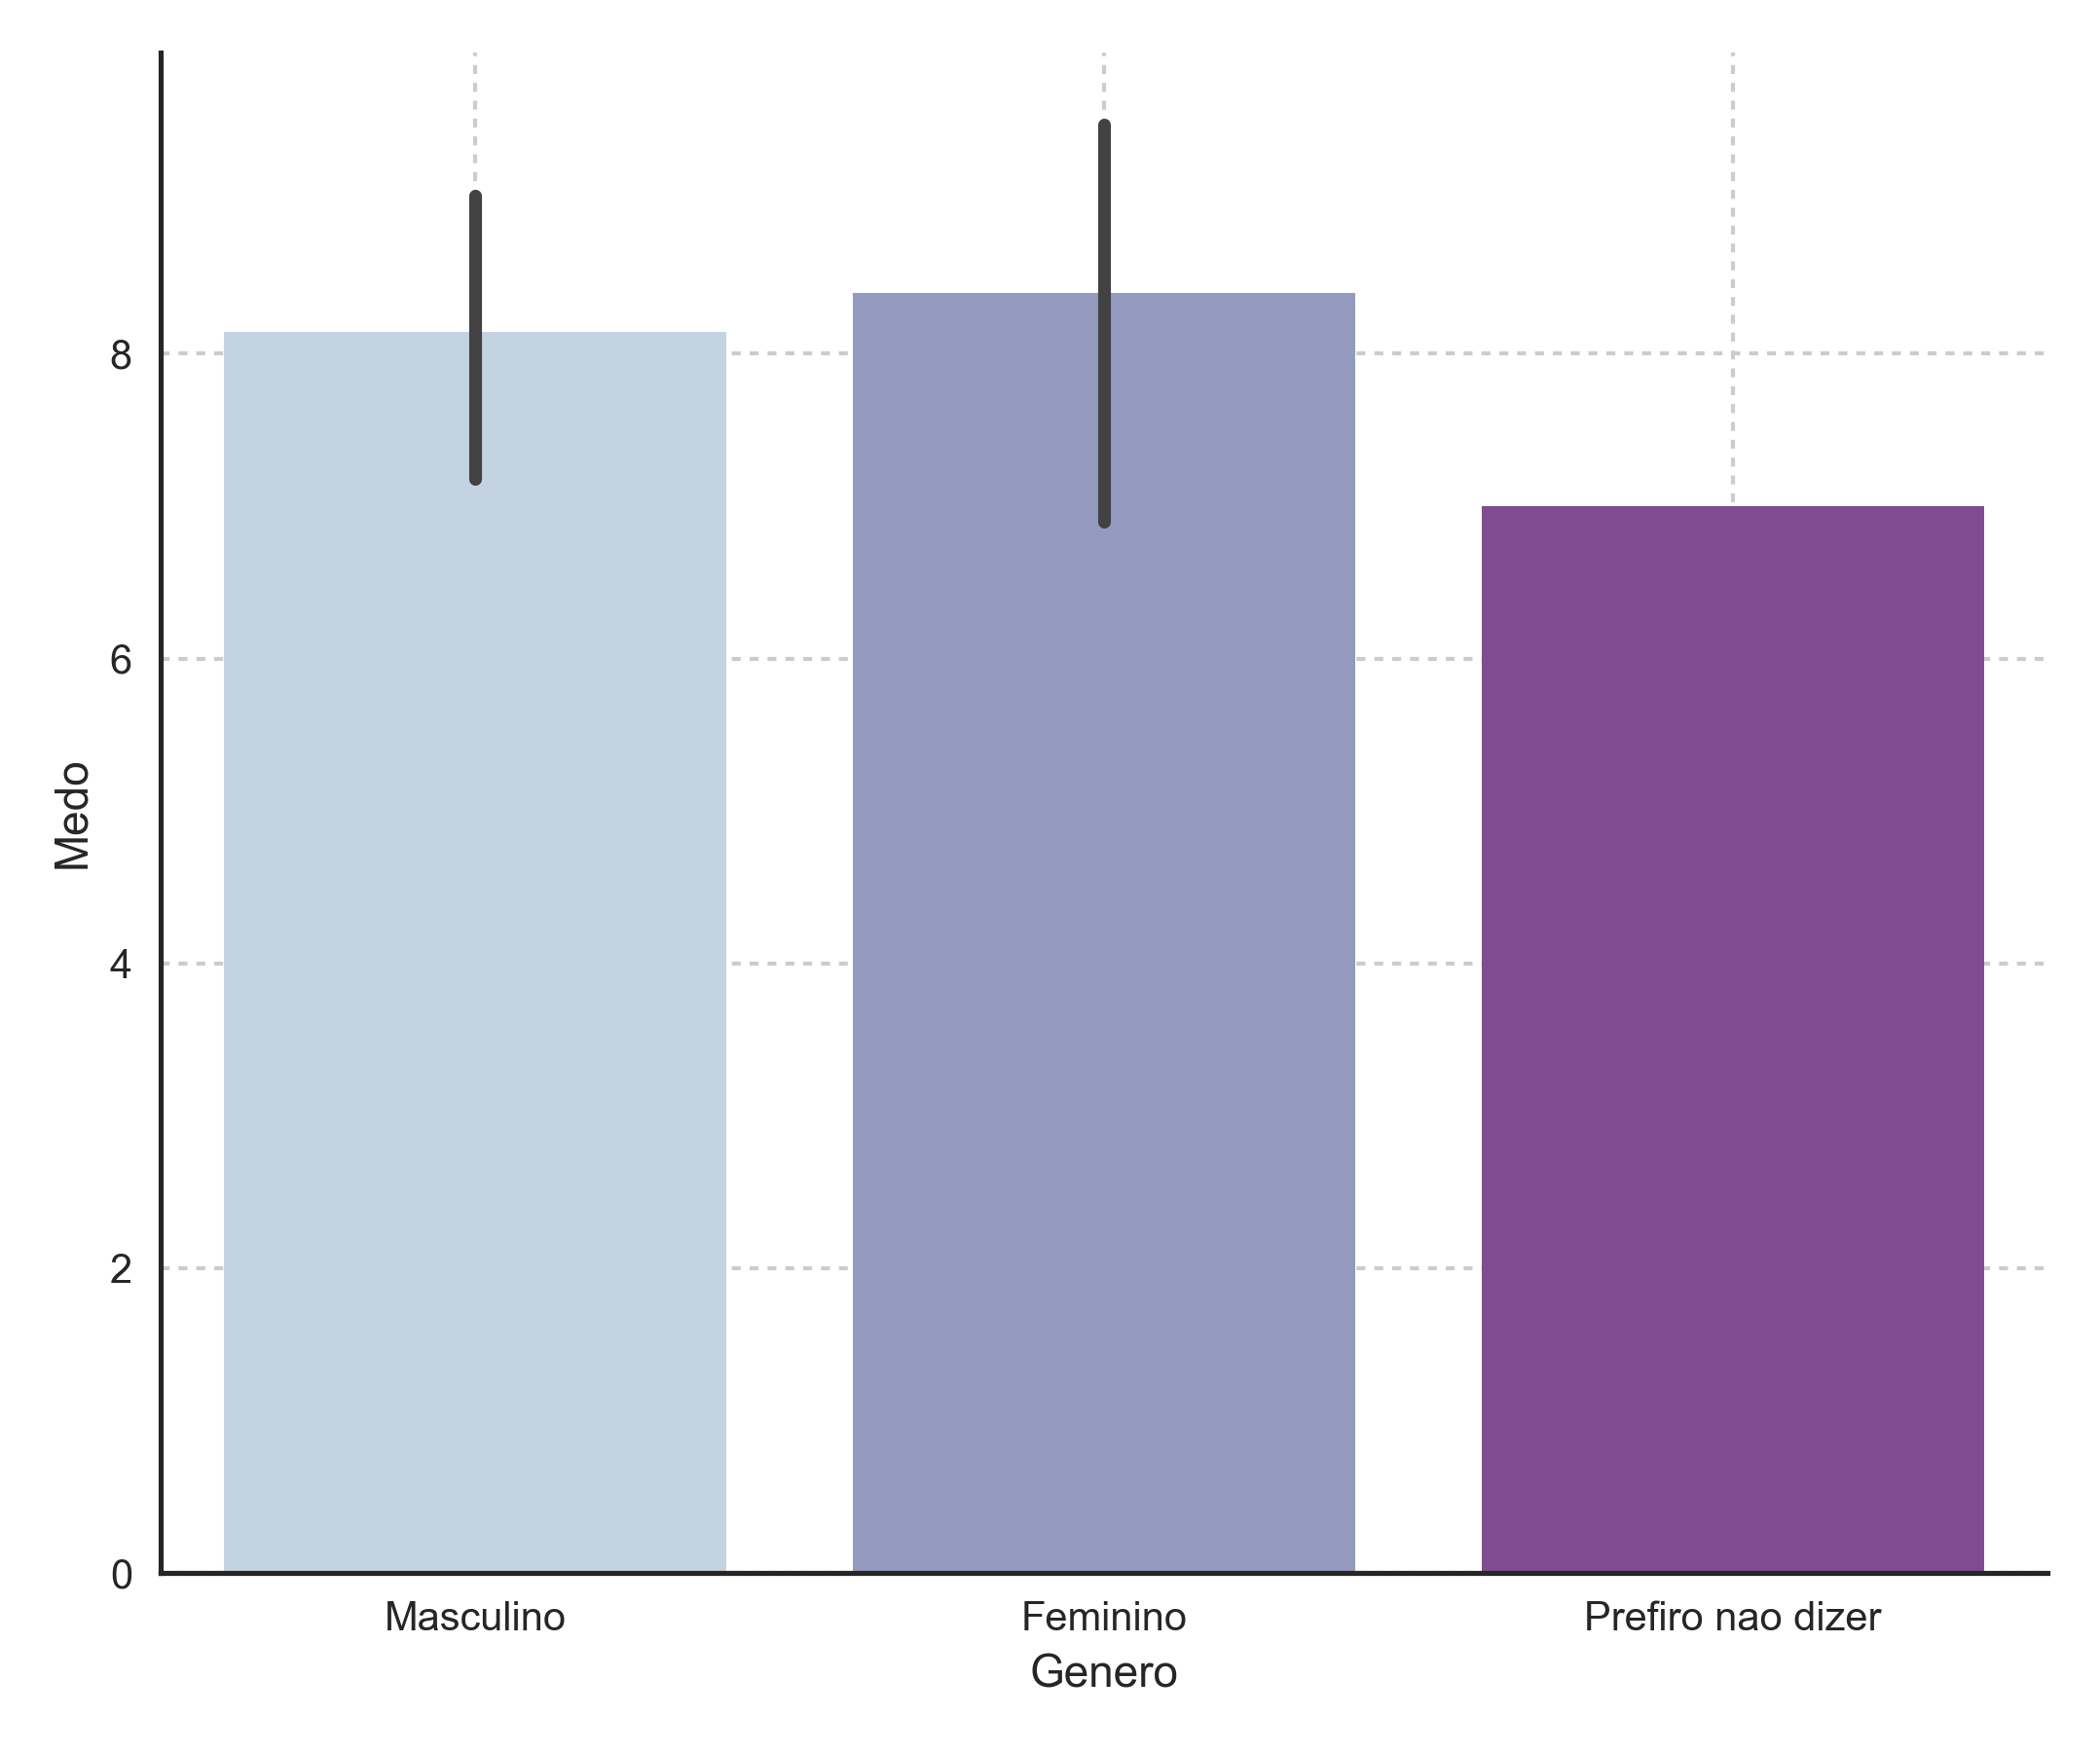
\includegraphics[width=\textwidth]{medo_genero.png}
		\smallcaption{Fonte: O autor.}
		\label{fig:medogenero}
	\end{minipage}
\end{figure}

Para a relação de medo e gênero, o que demonstrou menos medo foi o feminino. Isso era esperado devido ao resultado obtido sobre o conforto do usuário, apesar de nem sempre essa relação ser diretamente proporcional. A próxima análise é realizada com base na relação medo e idade, como demonstra a figura~\ref{fig:medoidade}.

\begin{figure}[ht!]
	\centering
	\begin{minipage}{0.65\textwidth}
		\caption{Medo por idade.}
		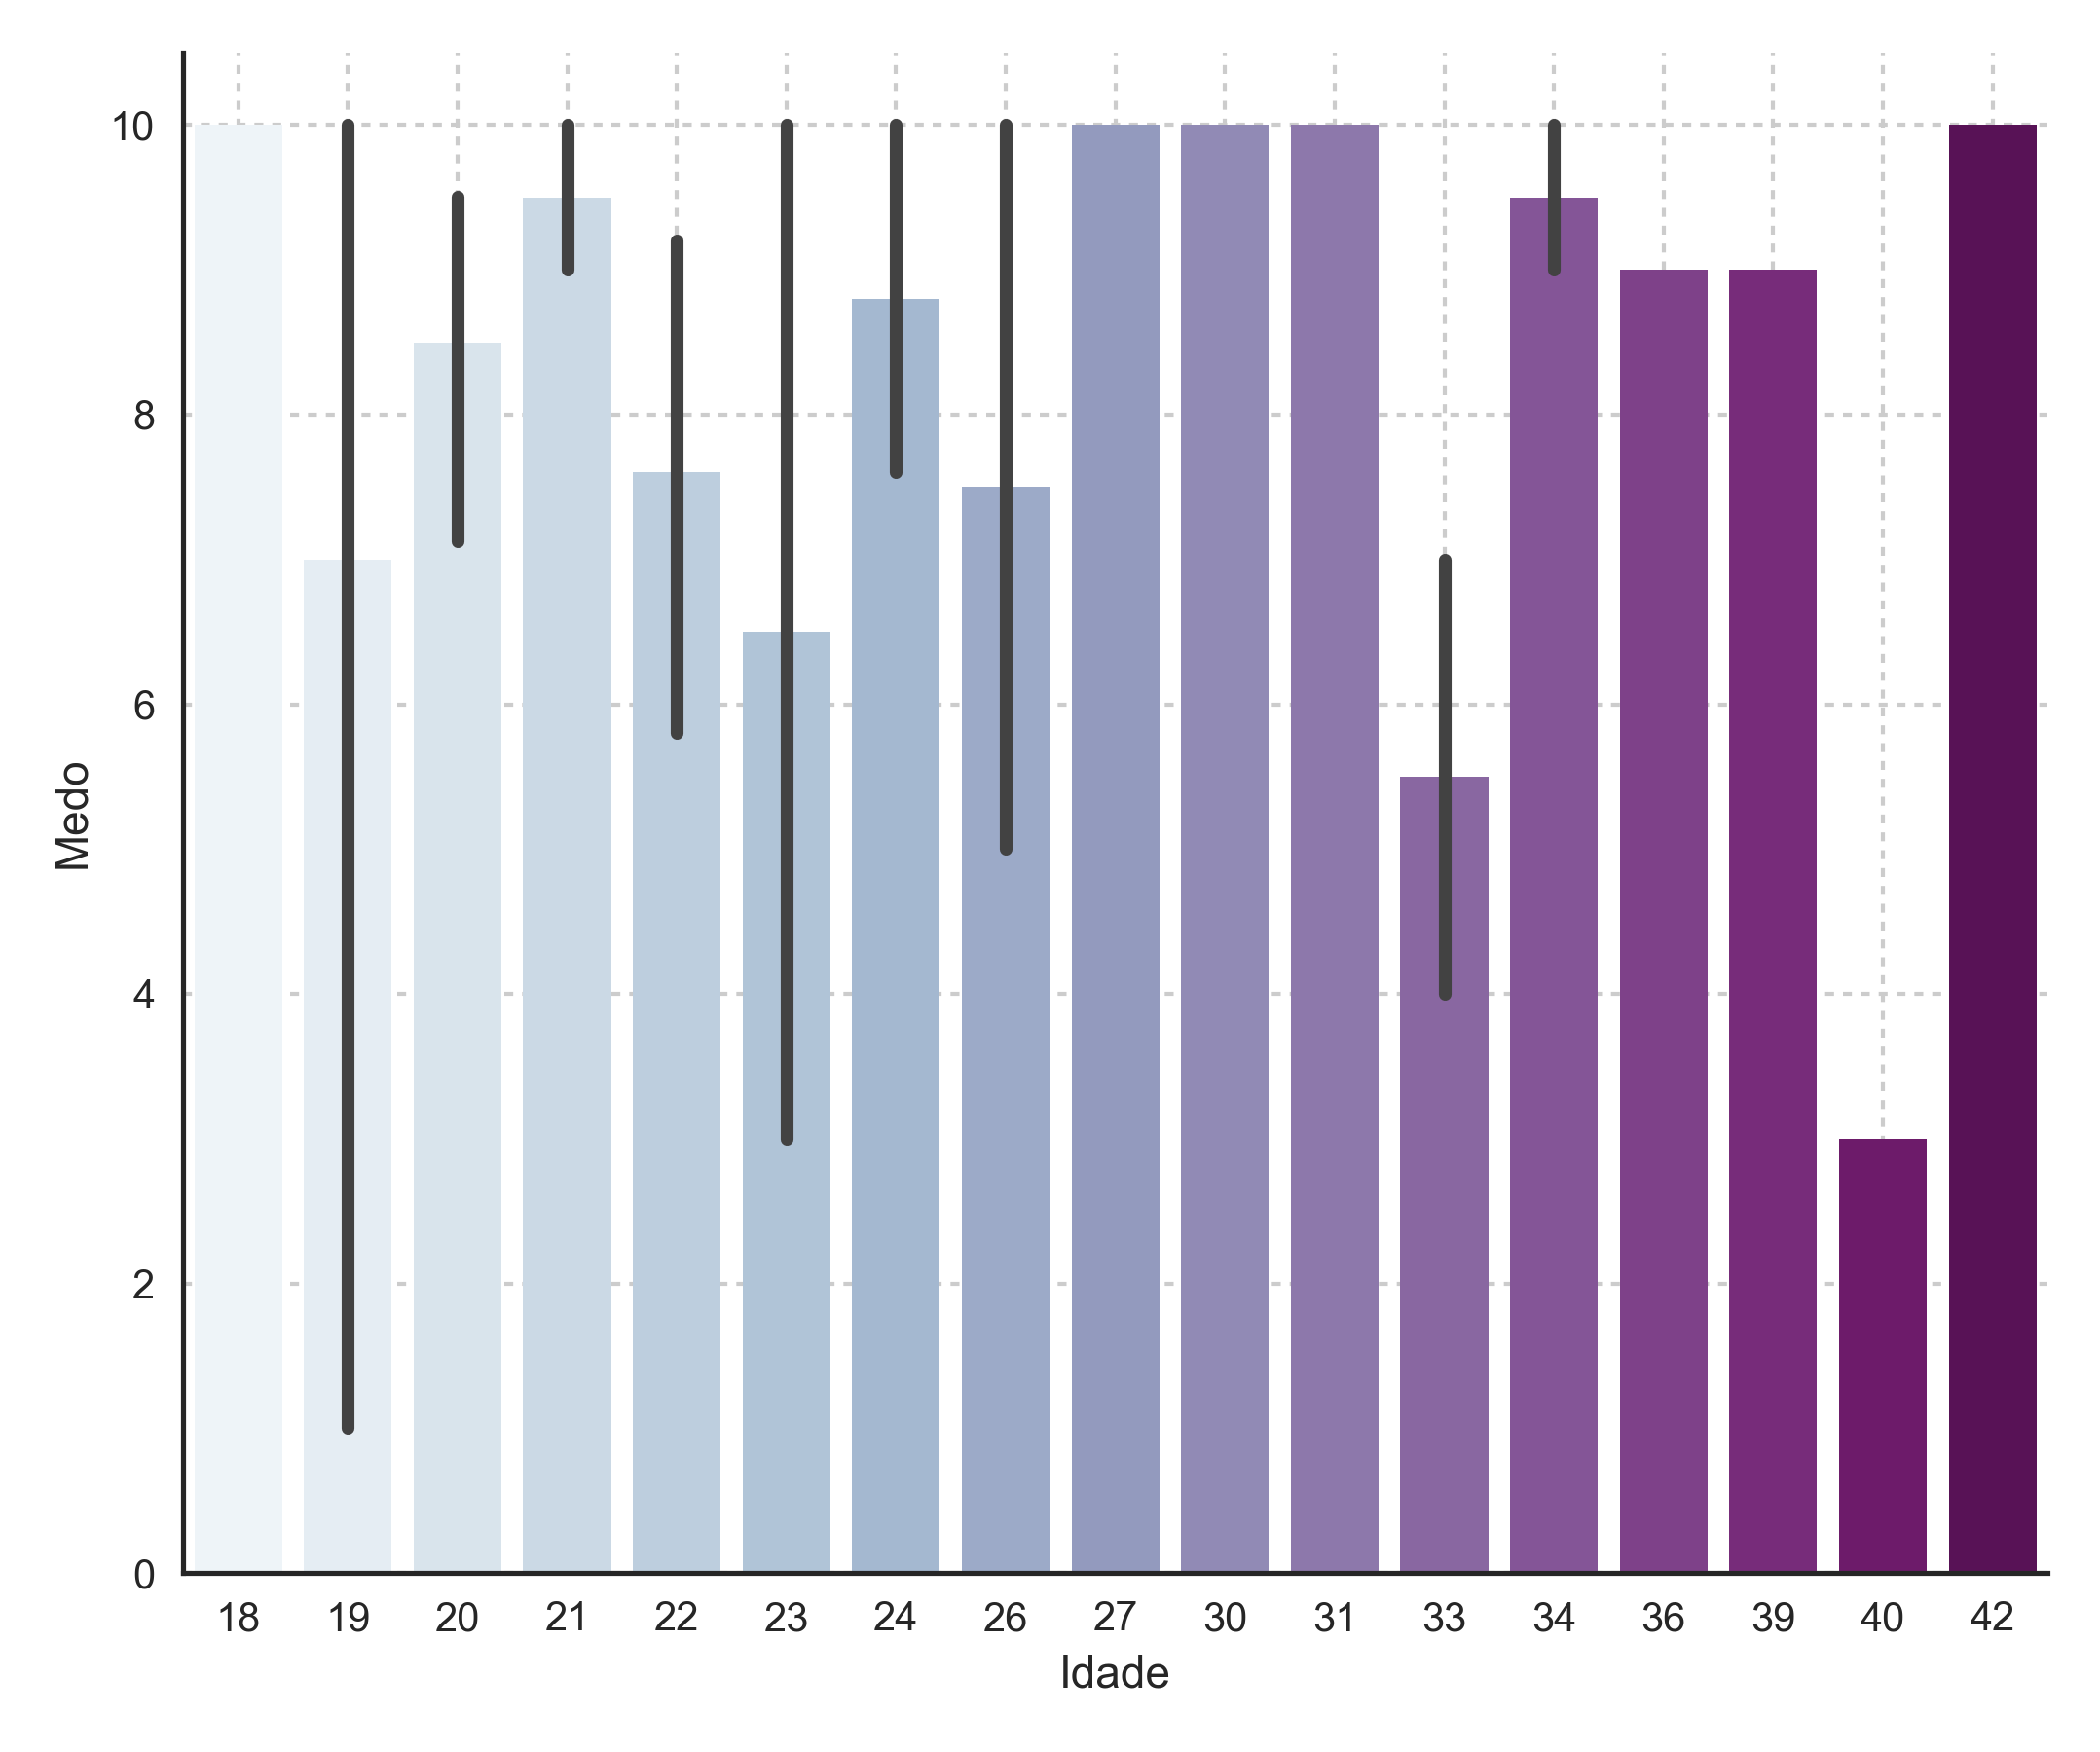
\includegraphics[width=\textwidth]{medo_idade.png}
		\smallcaption{Fonte: O autor.}
		\label{fig:medoidade}
	\end{minipage}
\end{figure}

A faixa etária com maior índice de medo foi os participantes de 40 anos. Um outro participante de 19 anos também apresentou um índice baixo sobre o medo do participante. Isso ocorreu, pois o comportamento invasivo do robô ao aproximar a garra deixou o participante assustado. Outro ponto levantado foi que o robô é muito barulhento.

\begin{figure}[ht!]
	\centering
	\begin{minipage}{0.65\textwidth}
		\caption{Medo por posição de interação.}
		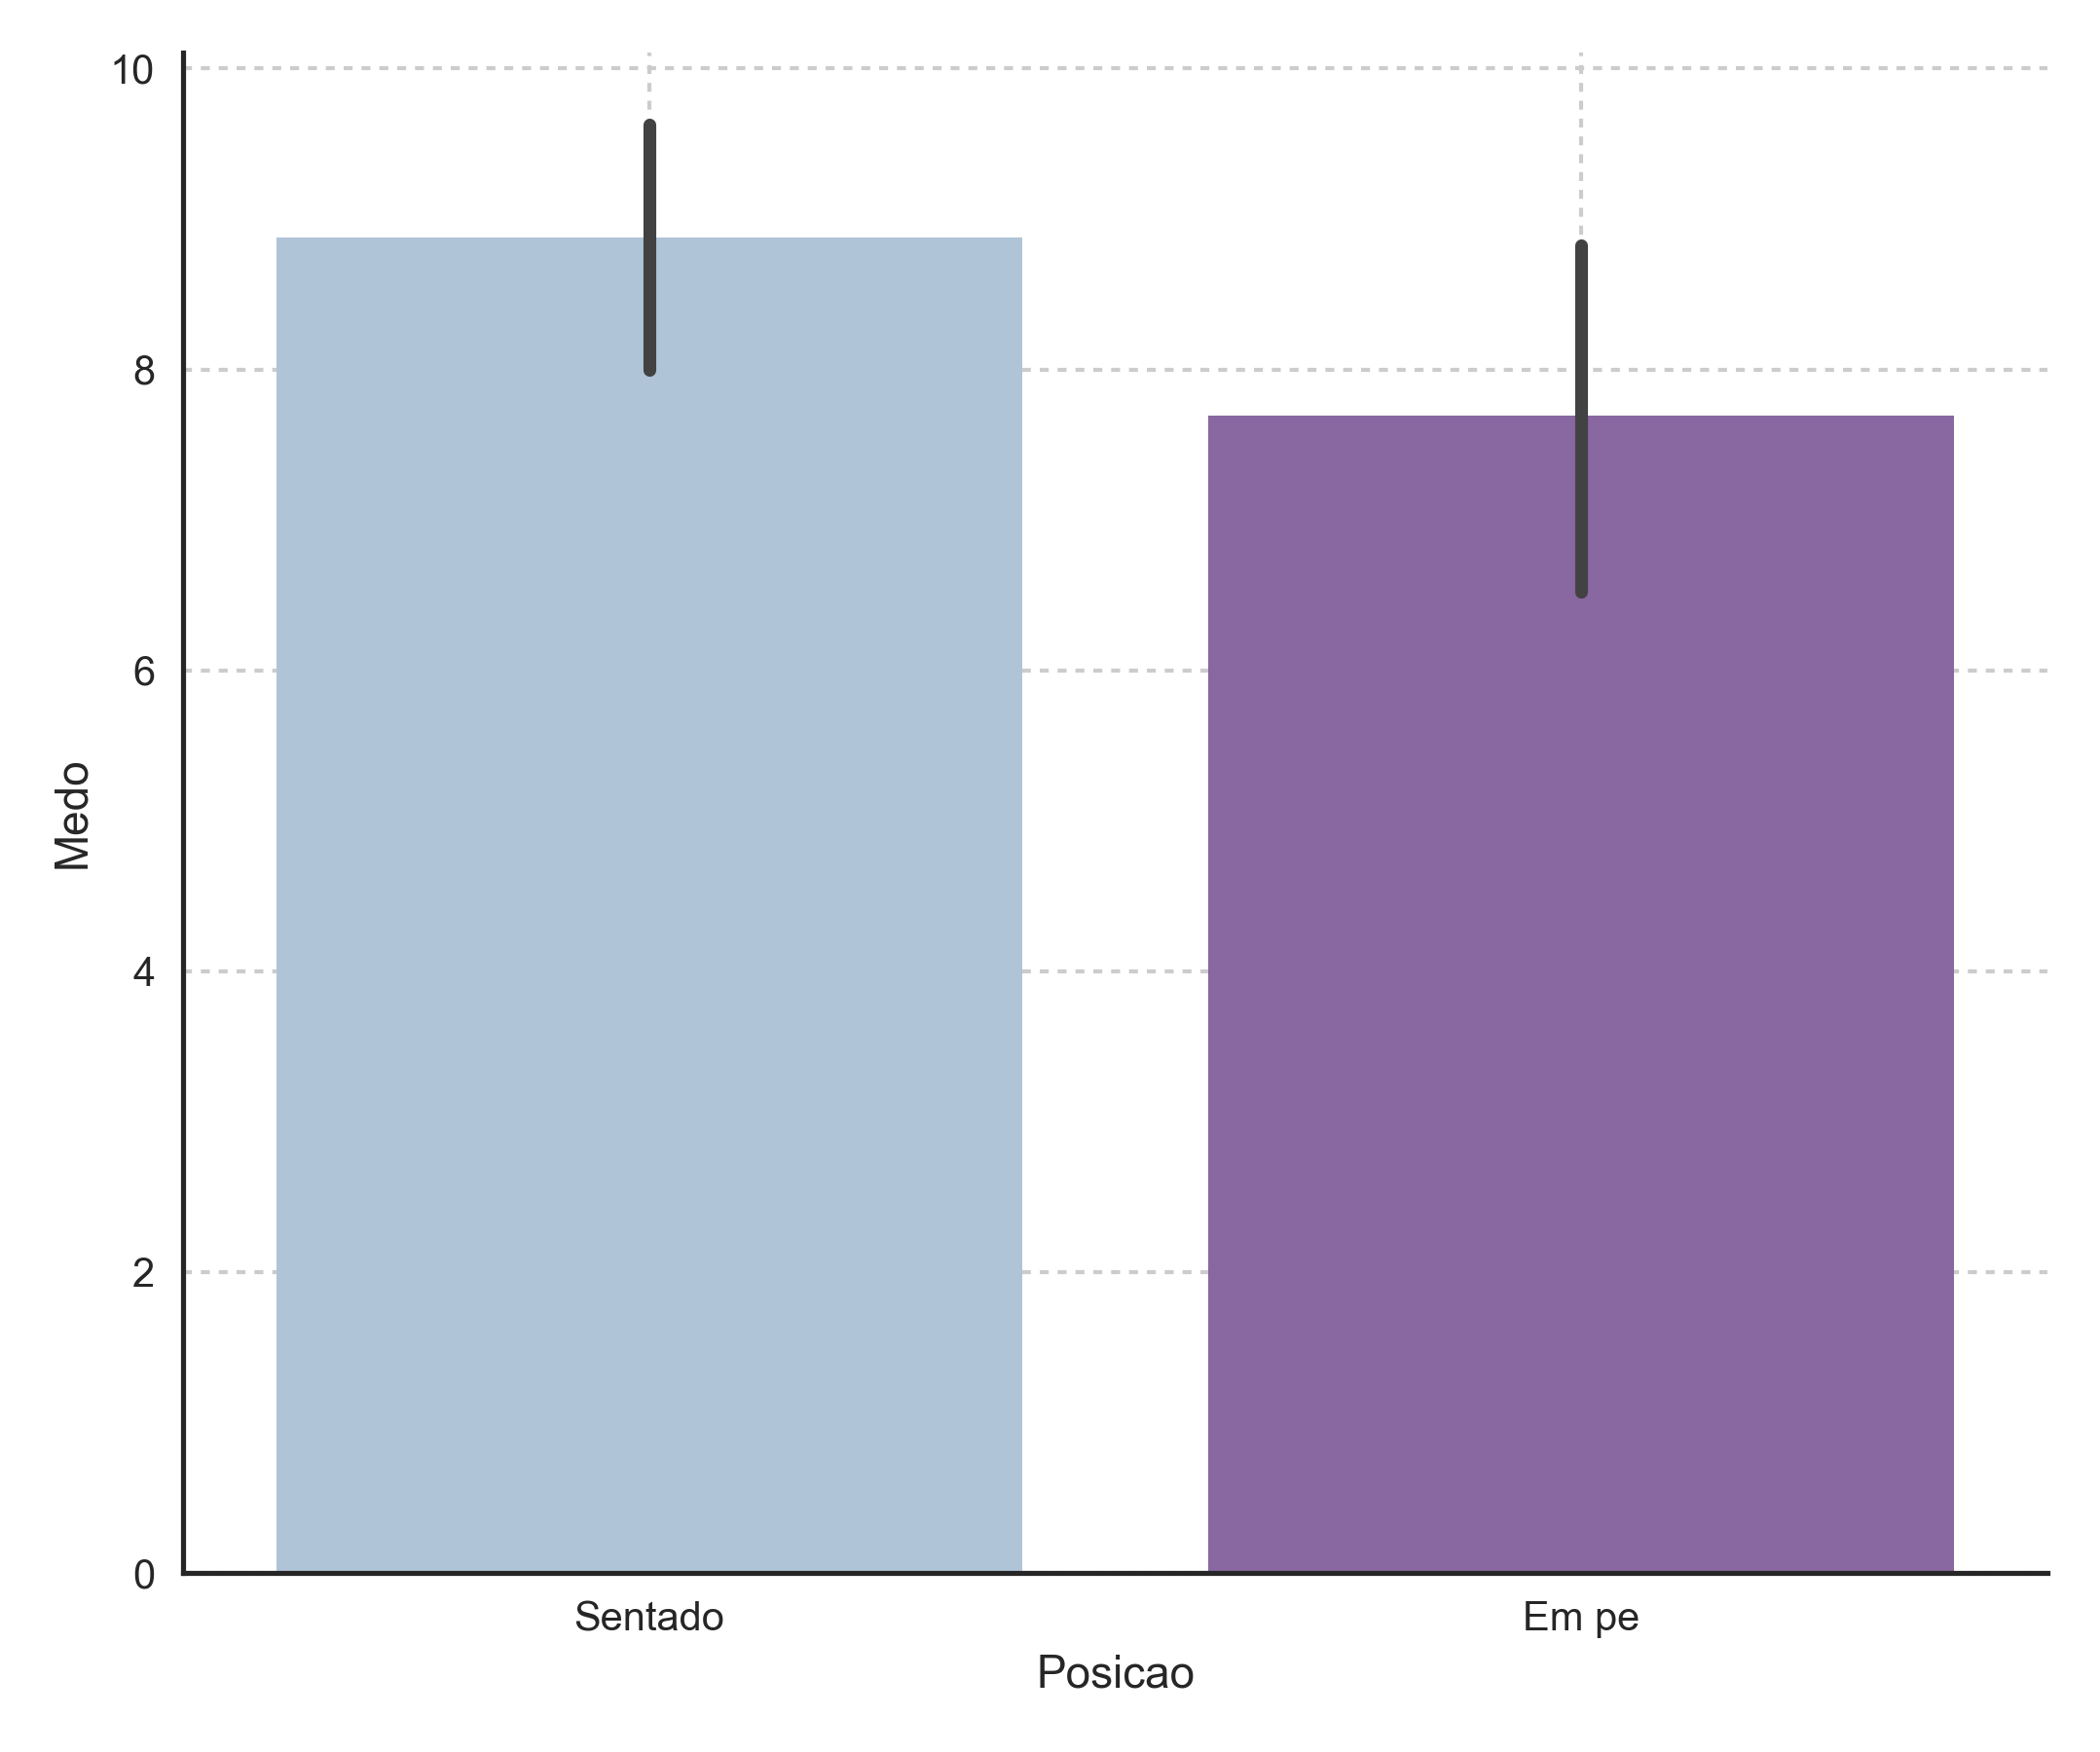
\includegraphics[width=\textwidth]{medo_posicao.png}
		\smallcaption{Fonte: O autor.}
		\label{fig:medoposicao}
	\end{minipage}
\end{figure}

\begin{figure}[ht!]
	\centering
	\begin{minipage}{0.65\textwidth}
		\caption{Medo por declaração de sociável.}
		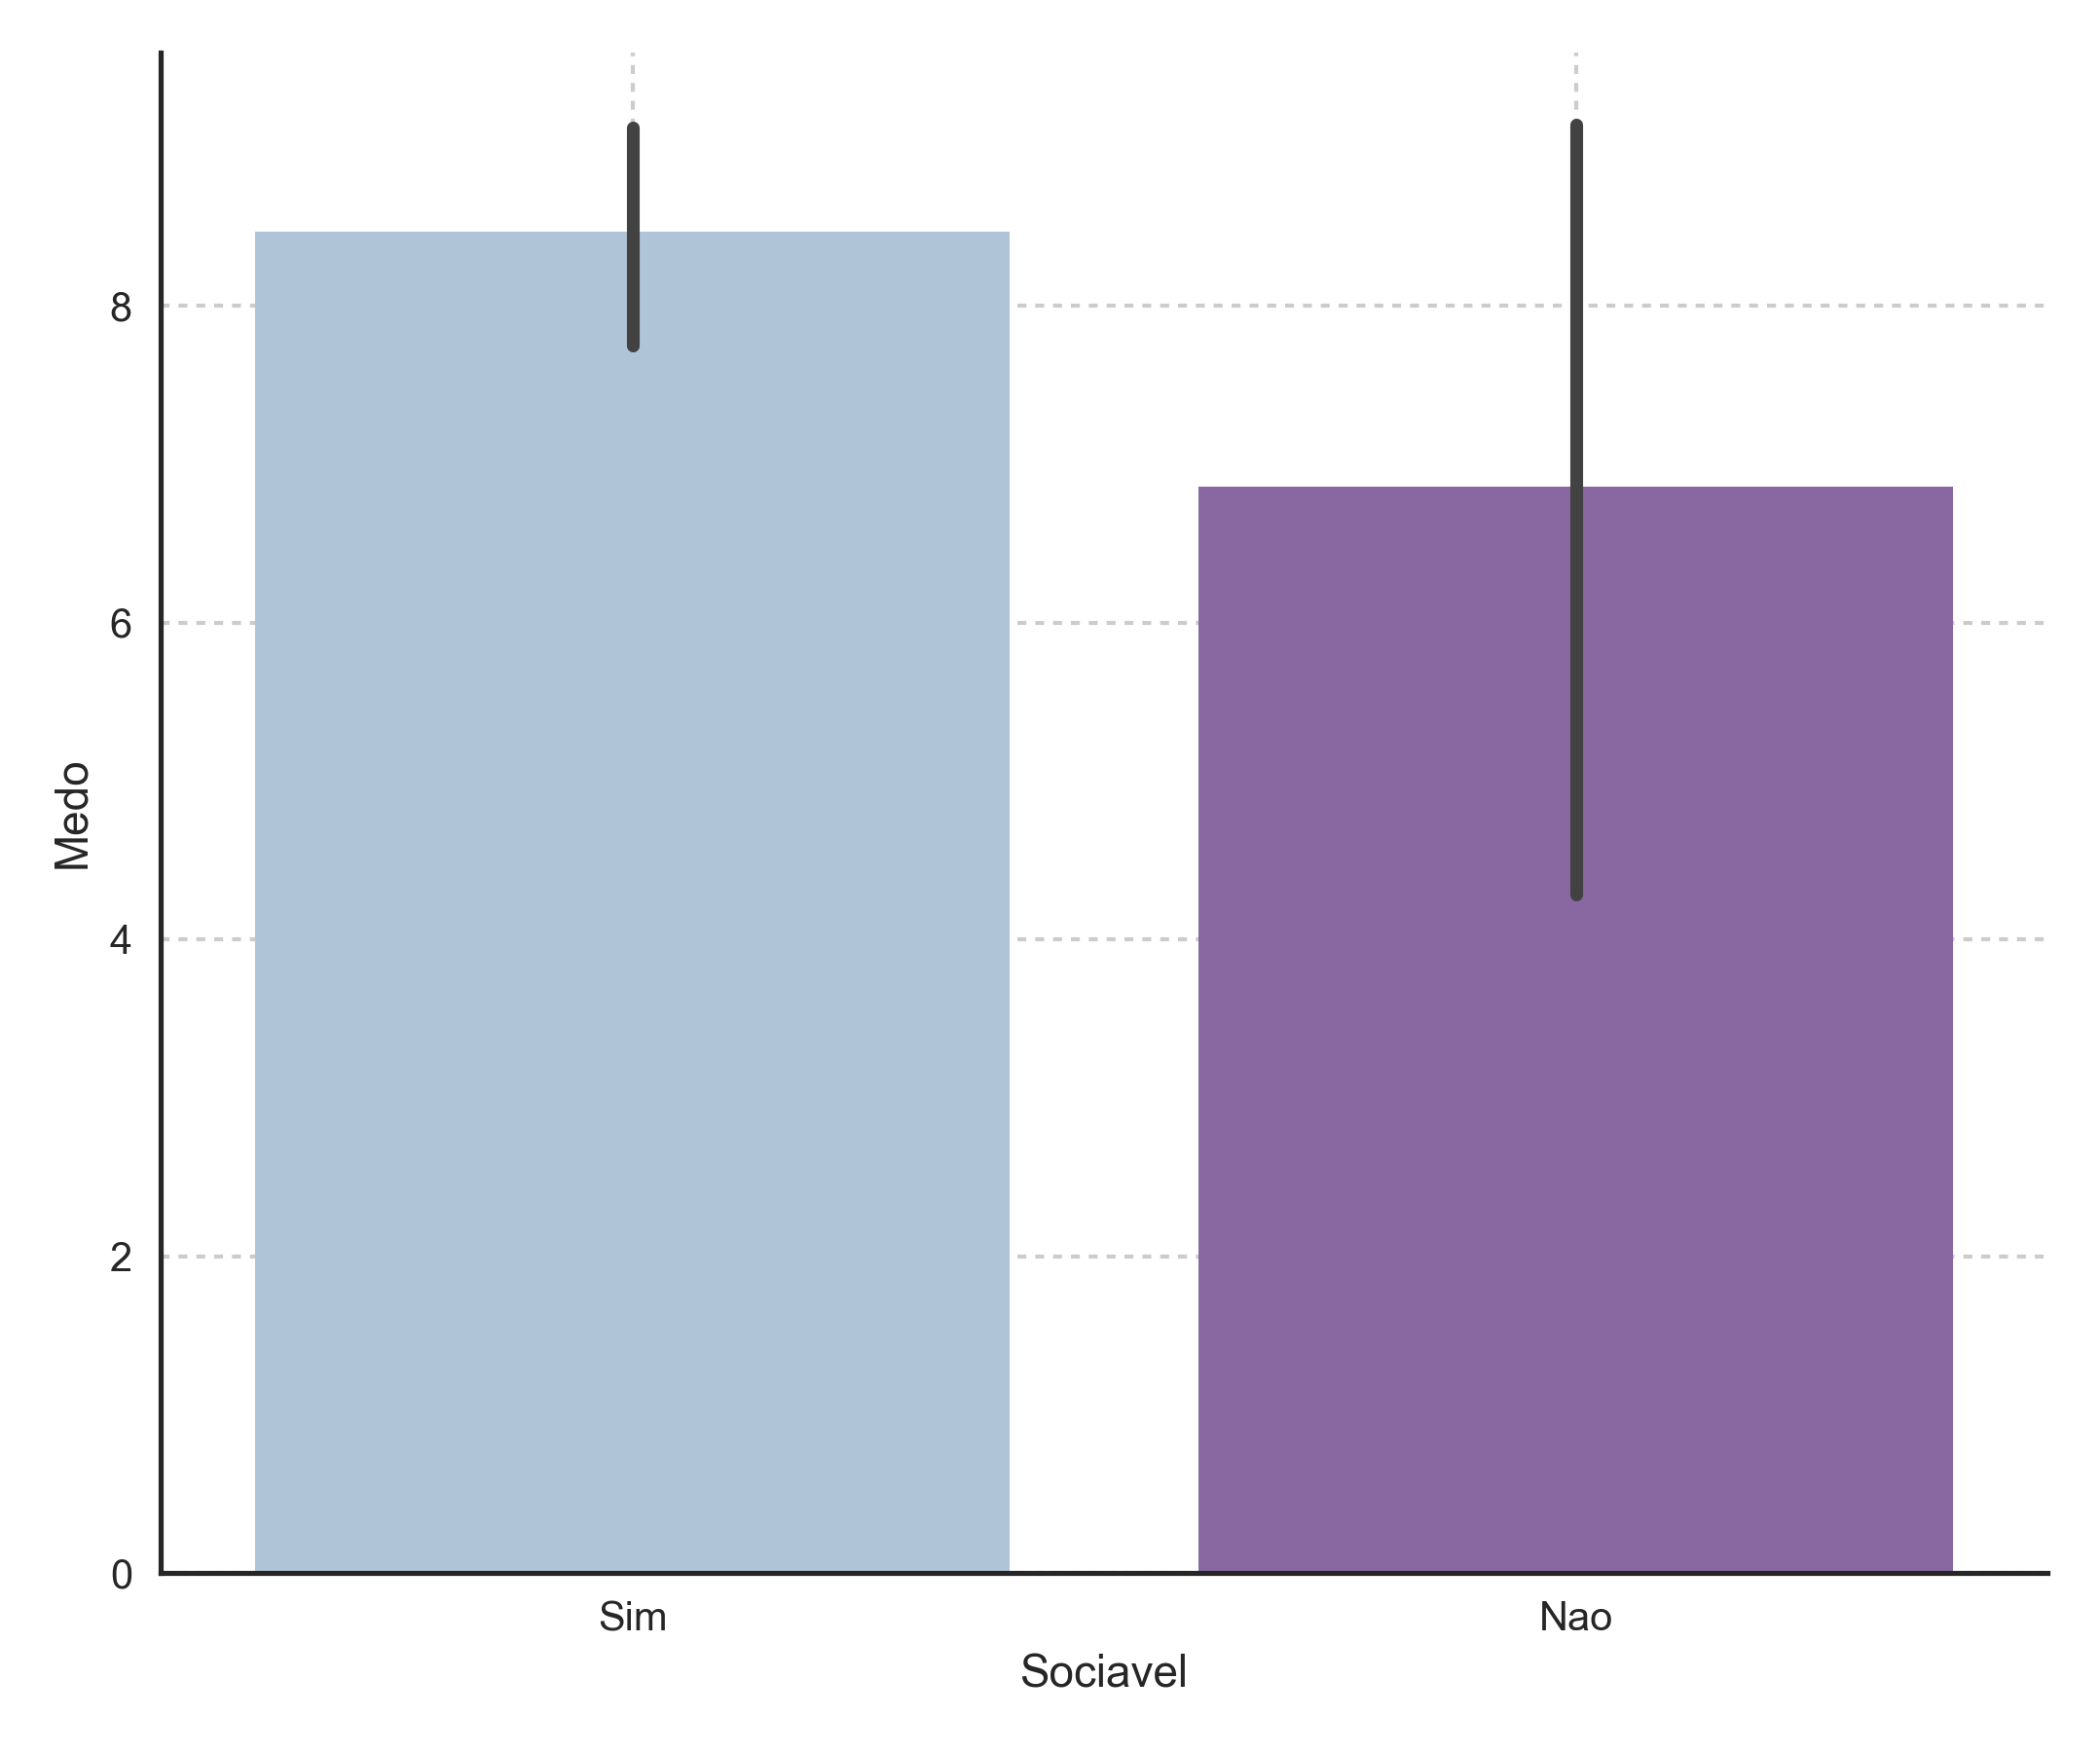
\includegraphics[width=\textwidth]{medo_sociavel.png}
		\smallcaption{Fonte: O autor.}
		\label{fig:medosociavel}
	\end{minipage}
\end{figure}
